A Gantt chart for the planned work is presented in Figure~\ref{fig:planning}. The planning is optimistic and the most risky section is the improvement of the code, in particular the addition of multiple revolution transfers. Thus, plenty of time has been allocated to these tasks.

\begin{figure}[htbp]
    \centering
    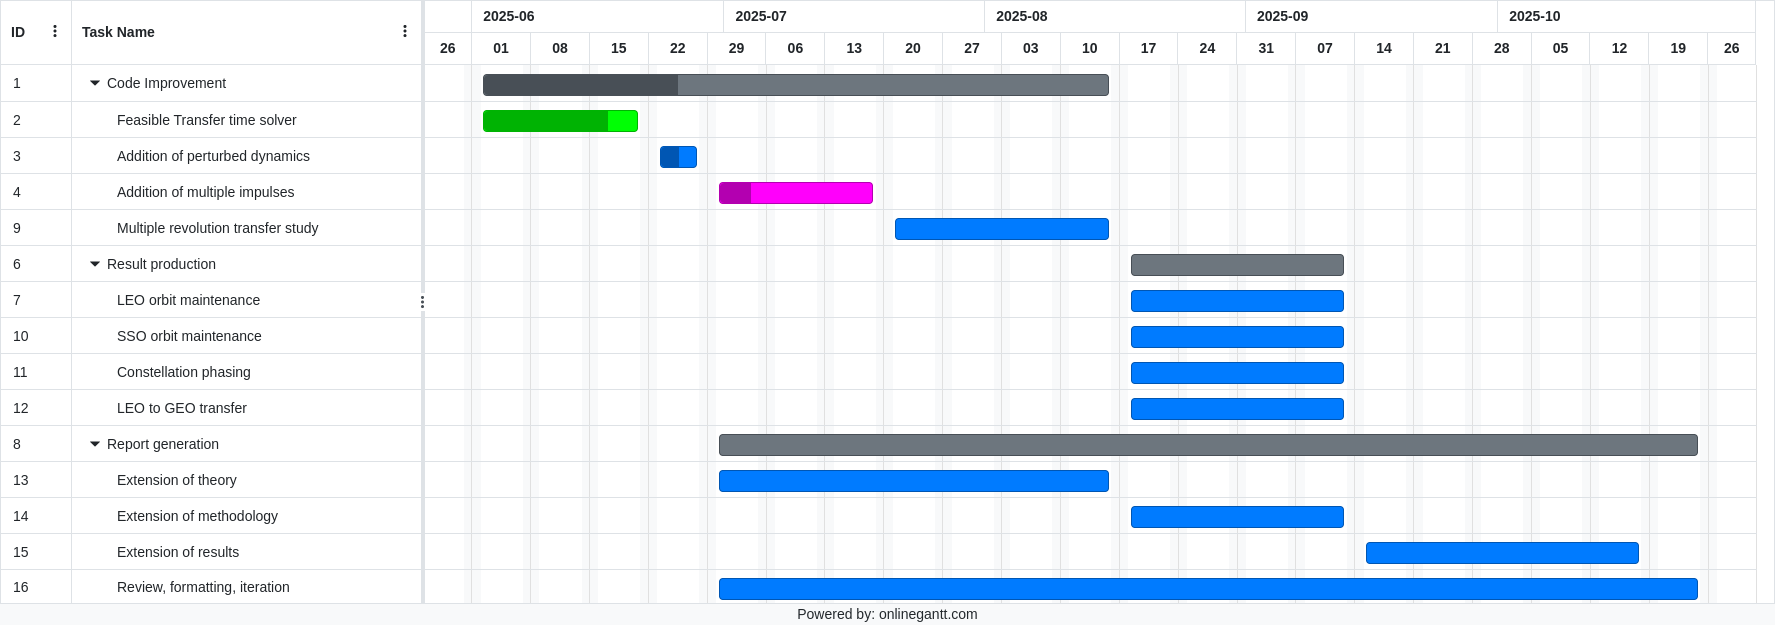
\includegraphics[width=\textwidth]{img/Planning.png}
    \caption{Gantt Chart of planned workload.}
    \label{fig:planning}
\end{figure}